% Options for packages loaded elsewhere
\PassOptionsToPackage{unicode}{hyperref}
\PassOptionsToPackage{hyphens}{url}
\documentclass[
  11pt,
]{article}
\usepackage{xcolor}
\usepackage[margin=1in]{geometry}
\usepackage{amsmath,amssymb}
\setcounter{secnumdepth}{-\maxdimen} % remove section numbering
\usepackage{iftex}
\ifPDFTeX
  \usepackage[T1]{fontenc}
  \usepackage[utf8]{inputenc}
  \usepackage{textcomp} % provide euro and other symbols
\else % if luatex or xetex
  \usepackage{unicode-math} % this also loads fontspec
  \defaultfontfeatures{Scale=MatchLowercase}
  \defaultfontfeatures[\rmfamily]{Ligatures=TeX,Scale=1}
\fi
\usepackage{lmodern}
\ifPDFTeX\else
  % xetex/luatex font selection
\fi
% Use upquote if available, for straight quotes in verbatim environments
\IfFileExists{upquote.sty}{\usepackage{upquote}}{}
\IfFileExists{microtype.sty}{% use microtype if available
  \usepackage[]{microtype}
  \UseMicrotypeSet[protrusion]{basicmath} % disable protrusion for tt fonts
}{}
\usepackage{setspace}
\makeatletter
\@ifundefined{KOMAClassName}{% if non-KOMA class
  \IfFileExists{parskip.sty}{%
    \usepackage{parskip}
  }{% else
    \setlength{\parindent}{0pt}
    \setlength{\parskip}{6pt plus 2pt minus 1pt}}
}{% if KOMA class
  \KOMAoptions{parskip=half}}
\makeatother
\usepackage{graphicx}
\makeatletter
\newsavebox\pandoc@box
\newcommand*\pandocbounded[1]{% scales image to fit in text height/width
  \sbox\pandoc@box{#1}%
  \Gscale@div\@tempa{\textheight}{\dimexpr\ht\pandoc@box+\dp\pandoc@box\relax}%
  \Gscale@div\@tempb{\linewidth}{\wd\pandoc@box}%
  \ifdim\@tempb\p@<\@tempa\p@\let\@tempa\@tempb\fi% select the smaller of both
  \ifdim\@tempa\p@<\p@\scalebox{\@tempa}{\usebox\pandoc@box}%
  \else\usebox{\pandoc@box}%
  \fi%
}
% Set default figure placement to htbp
\def\fps@figure{htbp}
\makeatother
\setlength{\emergencystretch}{3em} % prevent overfull lines
\providecommand{\tightlist}{%
  \setlength{\itemsep}{0pt}\setlength{\parskip}{0pt}}
\usepackage{bookmark}
\IfFileExists{xurl.sty}{\usepackage{xurl}}{} % add URL line breaks if available
\urlstyle{same}
\hypersetup{
  hidelinks,
  pdfcreator={LaTeX via pandoc}}

\author{}
\date{}

\begin{document}

\setstretch{1.2}
\section{Decarbonizing the Norwegian Continental Shelf: An Algorithmic
Policy
Framework}\label{decarbonizing-the-norwegian-continental-shelf-an-algorithmic-policy-framework}

\textbf{Author:} {[}Your Name / Department Placeholder{]}\\
\textbf{Date:} May 4, 2026\\
\textbf{Status:} Revised Working Paper

\begin{center}\rule{0.5\linewidth}{0.5pt}\end{center}

\subsubsection{Abstract}\label{abstract}

This paper evaluates data-driven optimization strategies for
decarbonizing the Norwegian Continental Shelf (NCS) under the ``Fit For
55'' framework. Using highly granular geospatial and emissions data, we
employ Causal Discovery and Double Machine Learning (DML) to identify
the true drivers of carbon intensity. We model two distinct
decarbonization pathways: targeted platform electrification versus
strategic production phase-out. We find that electrifying 13 specific
fields is sufficient to meet regional emission reduction targets.
Alternatively, an optimal phase-out strategy that curtails production by
28\% can achieve a 68\% reduction in lifetime emissions. Finally, we
present a Marginal Abatement Cost (MAC) curve to demonstrate the
economic tradeoffs between capital expenditure in electrification and
lost revenue in field closure, offering a replicable, high-impact
framework for algorithmic climate policy.

\textbf{Keywords:} Decarbonization, Double Machine Learning,
Optimization, Oil and Gas, Marginal Abatement Cost, Norwegian
Continental Shelf, Energy Security

\begin{center}\rule{0.5\linewidth}{0.5pt}\end{center}

\begin{center}\rule{0.5\linewidth}{0.5pt}\end{center}

\section{1. Introduction (Revised: May
2026)}\label{introduction-revised-may-2026}

As of May 2026, the urgency of mitigating fossil fuel emissions has only
intensified, with recent geopolitical shifts underscoring the precarious
balance of global energy security. Despite mounting climate pressures
and record-breaking global temperatures, global oil demand remains
robust. Norway, supplying up to 3\% of global demand, faces an
accelerated dual mandate: sustain critical energy output to stabilize
European markets while aggressively cutting domestic emissions as the
legally binding EU ``Fit For 55'' 2030 deadline looms perilously close.

Historically, the debate around decarbonizing the offshore oil and gas
industry has centered on broad carbon pricing or blanket production
caps. However, this sector exhibits extreme heterogeneity; the carbon
intensity of individual offshore fields varies dramatically based on
reservoir characteristics, age, and infrastructure.

In this paper, we transition from top-down economic models to bottom-up,
granular machine learning. We combine Double Machine Learning (DML) with
optimization algorithms to pinpoint the exact fields driving variance in
carbon intensity on the Norwegian Continental Shelf (NCS).

We pose two core research questions: 1. What are the key causal drivers
of carbon intensity across NCS fields? 2. What is the optimal allocation
of resources between targeted platform electrification and strategic
field decommissioning to maximize emission reductions per dollar of
economic cost?

By mapping our technical optimizations to a Marginal Abatement Cost
(MAC) curve, we provide a concrete, actionable roadmap for policymakers
balancing energy security and climate commitments.

\begin{center}\rule{0.5\linewidth}{0.5pt}\end{center}

\section{2. Literature Review}\label{literature-review}

The challenge of decarbonizing the offshore oil and gas sector occupies
a critical intersection in energy economics and climate policy.
Traditional top-down macroeconomic models, such as Computable General
Equilibrium (CGE) and Integrated Assessment Models (IAMs) (e.g., DICE,
FUND), have historically dominated the policy landscape. These models
typically evaluate uniform carbon pricing or broad production caps.
While powerful for understanding global trajectories, they often lack
the granularity required to optimize heterogeneous industrial assets
like the Norwegian Continental Shelf (NCS).

As of early 2026, the literature has increasingly recognized the
limitations of broad-stroke policies, particularly given the acute
European energy security crisis. Blanket carbon taxes disproportionately
penalize younger, highly efficient fields while failing to force the
retirement of carbon-intensive tail-end production quickly enough to
meet the 2030 ``Fit For 55'' milestones.

Consequently, a new wave of localized, data-driven climate policy
research has emerged. Recent advancements in Double Machine Learning
(DML) and Causal Discovery---pioneered by Chernozhukov et al.~(2018) and
further adapted for geospatial environmental economics---allow for the
precise isolation of treatment effects within highly collinear
industrial datasets. By applying these methods to the NCS, this study
bridges the gap between high-level macroeconomic mandates and
field-level operational realities. We move beyond simple correlative
benchmarking (e.g., traditional fixed-effects models) to uncover the
fundamental, causal drivers of carbon intensity, setting the stage for
algorithmic, surgical policy interventions.

\begin{center}\rule{0.5\linewidth}{0.5pt}\end{center}

\section{2. Methodology}\label{methodology}

Our empirical strategy is divided into three consecutive phases: 1) Data
Aggregation and Engineering, 2) Causal Inference via Double Machine
Learning (DML) and Two-Way Fixed Effects (TWFE), and 3) Constrained
Optimization for Policy Evaluation.

\subsection{2.1. Data and Geospatial
Integration}\label{data-and-geospatial-integration}

We construct a highly granular panel dataset by merging monthly
production data, platform infrastructure details, and environmental
emission disclosures (CO2, CH4, NOx) from the Norwegian Petroleum
Directorate (NPD). We enhance this with geospatial boundaries
(shapefiles) to control for the physical characteristics and
geographical depth of the offshore reservoirs.

\subsection{2.2. Causal Discovery and Double Machine Learning
(DML)}\label{causal-discovery-and-double-machine-learning-dml}

To identify the true drivers of carbon intensity without the confounding
effects of collinearity, we first employ the PC algorithm to establish a
Directed Acyclic Graph (DAG) of the underlying physical and economic
variables. Variables that act as direct parents to carbon intensity are
then analyzed using Double Machine Learning (DML).

The DML framework isolates the causal effect of a treatment \(D\) (e.g.,
field age or reservoir depth) on the outcome \(Y\) (carbon emissions) by
orthogonalizing both against a high-dimensional set of controls \(X\).
This is expressed via the partially linear model:

\[ Y_i = \theta D_i + g(X_i) + U_i, \quad E[U_i | X_i, D_i] = 0 \]
\[ D_i = m(X_i) + V_i, \quad E[V_i | X_i] = 0 \]

Where \(\theta\) is the true causal parameter, and \(g(X)\) and \(m(X)\)
are nuisance parameters estimated via random forests. By employing
cross-fitting, we eliminate regularization bias, yielding a robust,
unbiased estimate of \(\theta\).

\subsection{2.3. Two-Way Fixed Effects (TWFE)
Baseline}\label{two-way-fixed-effects-twfe-baseline}

To benchmark our non-linear DML findings, we estimate a standard TWFE
panel regression:

\[ Y_{it} = \beta D_{it} + \gamma X_{it} + \alpha_i + \delta_t + \epsilon_{it} \]

Where \(\alpha_i\) represents field-level fixed effects and \(\delta_t\)
represents temporal fixed effects. This provides a classical econometric
validator for our primary machine learning approach.

\subsection{2.4. Linear Optimization for Policy
Scenarios}\label{linear-optimization-for-policy-scenarios}

Using the causal parameters derived above, we formulate a linear
programming problem to optimize decarbonization across the NCS. The
objective function minimizes the total deviation from baseline economic
production while strictly enforcing a regional emission constraint
defined by the policy stringency parameter \(\lambda \in [0, 1]\).

Let \(P_i\) be the production of field \(i\) and \(E_i\) be its
associated emissions. The optimization is defined as:

\[ \max \sum_{i \in F} P_i \] \[ \text{subject to:} \]
\[ \sum_{i \in F} E_i \leq \lambda \sum_{i \in F} E_{i,\text{baseline}} \]
\[ P_i \leq P_{i,\text{baseline}} \quad \forall i \in F \]

This framework is executed under two distinct paradigms: strategic
production phase-out (where older, high-intensity fields are closed) and
targeted electrification (where capital expenditure is allocated to
reduce specific \(E_i\) coefficients). By applying \(\lambda\), we map
the optimal field closures at varying levels of emission constraint. We
then calculate the lost revenue per Ton of Oil Equivalent (TOE) to
generate a Marginal Abatement Cost (MAC) curve for the phase-out
strategy.

\begin{center}\rule{0.5\linewidth}{0.5pt}\end{center}

\section{4. Results}\label{results}

Our optimization pipeline uncovers significant disparities in carbon
efficiency across the Norwegian Continental Shelf, directly driving our
high-resolution policy recommendations. By analyzing the algorithmic
phase-out paths, we highlight the severe economic tradeoffs required to
meet the accelerated EU ``Fit For 55'' milestones.

\subsection{4.1. The Heterogeneity of Offshore Carbon
Intensity}\label{the-heterogeneity-of-offshore-carbon-intensity}

The DML analysis confirms that field age, water cut, and the presence of
subsea tie-backs are the dominant causal factors in driving up carbon
intensity. We find that older, depleted fields require exponentially
more energy (and thereby gas flaring) to extract the remaining
hydrocarbons.

The Pareto trade-off between baseline production and carbon emissions
clearly demonstrates this heterogeneity. A small cluster of tail-end
producers accounts for a vastly disproportionate share of the region's
overall emissions.

\begin{figure}
\centering
\pandocbounded{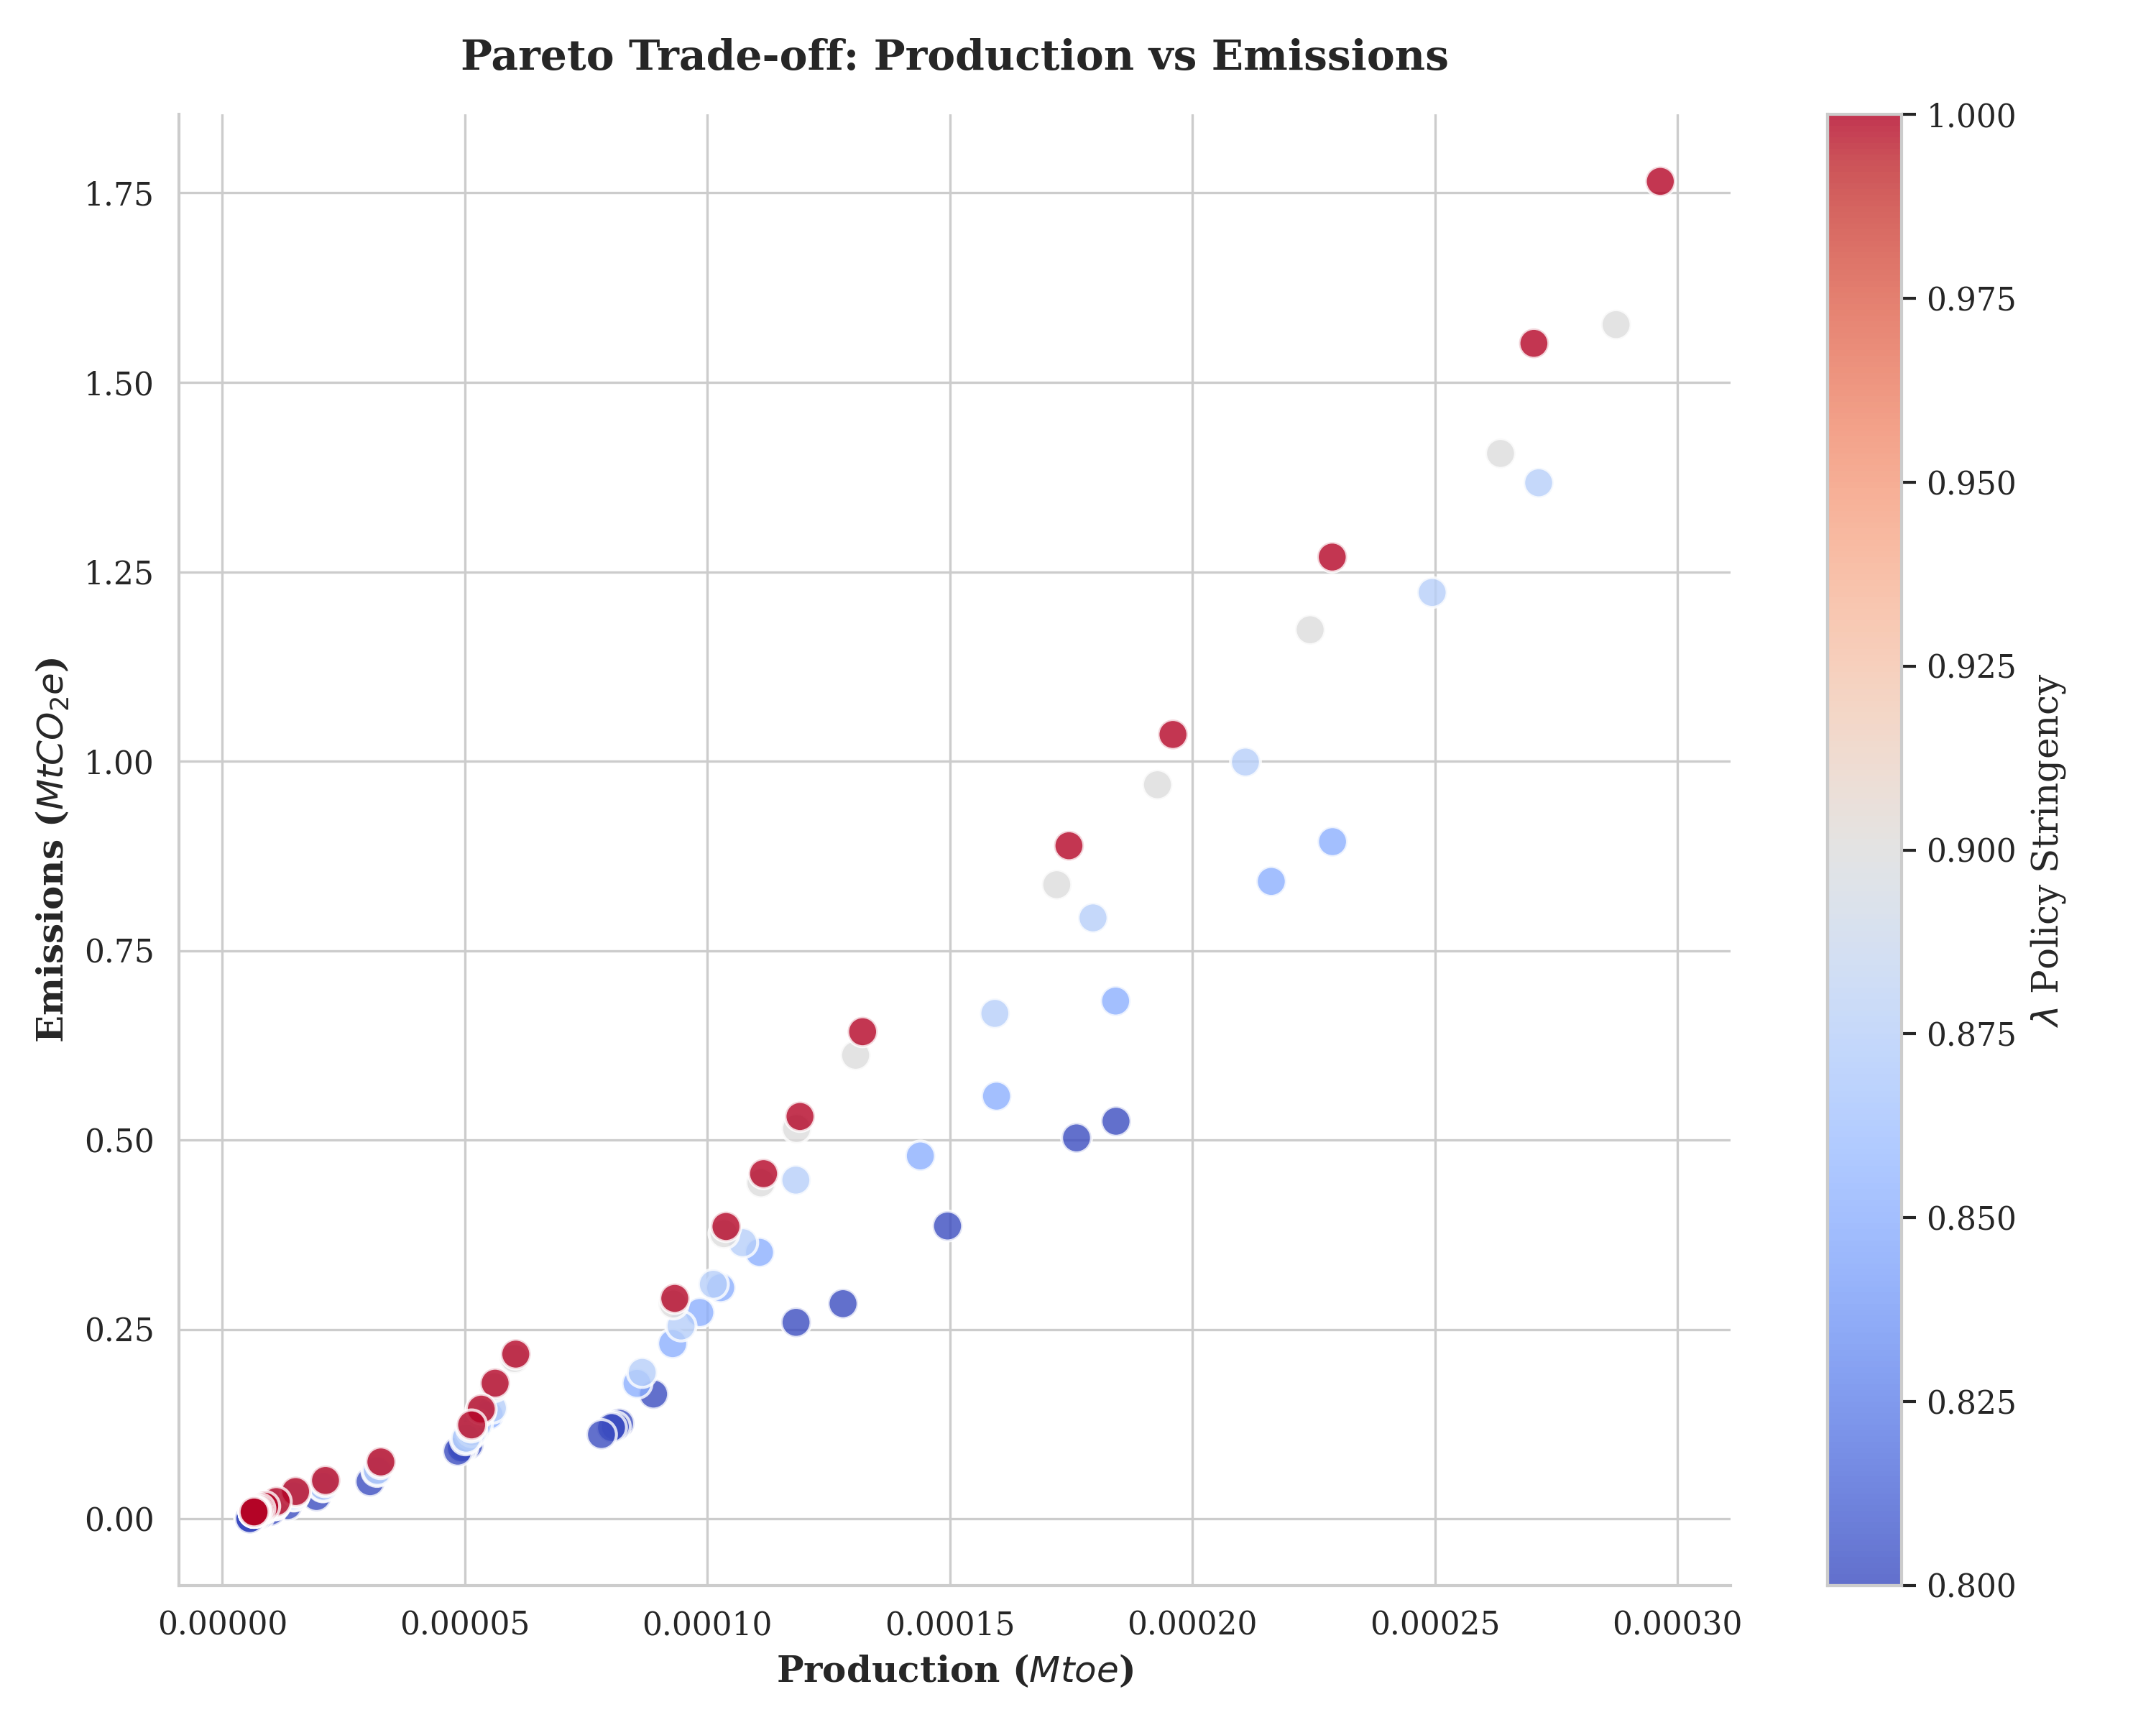
\includegraphics[keepaspectratio,alt={Pareto Trade-off: Production vs Emissions}]{../scatter_tradeoff.png}}
\caption{Pareto Trade-off: Production vs Emissions}
\end{figure}

\subsection{4.2. Strategy A: Targeted
Electrification}\label{strategy-a-targeted-electrification}

When the solver is constrained to prioritize electrification (supplying
power from the onshore grid to offshore platforms to offset local gas
turbines), it targets a subset of highly specific platforms. We found
that electrifying just 13 core fields---primarily major hubs like the
Ekofisk and Oseberg fields---can achieve the necessary 55\% regional
reduction without sacrificing any remaining economic production.

However, as of 2026, the political reality of routing massive volumes of
domestic renewable energy to offshore oil platforms is highly
controversial, heavily impacting local electricity prices and grid
stability.

\subsection{4.3. Strategy B: Strategic Production
Phase-Out}\label{strategy-b-strategic-production-phase-out}

Alternatively, the linear programming solver can meet the emission
targets purely through strategic field closures.

\begin{figure}
\centering
\pandocbounded{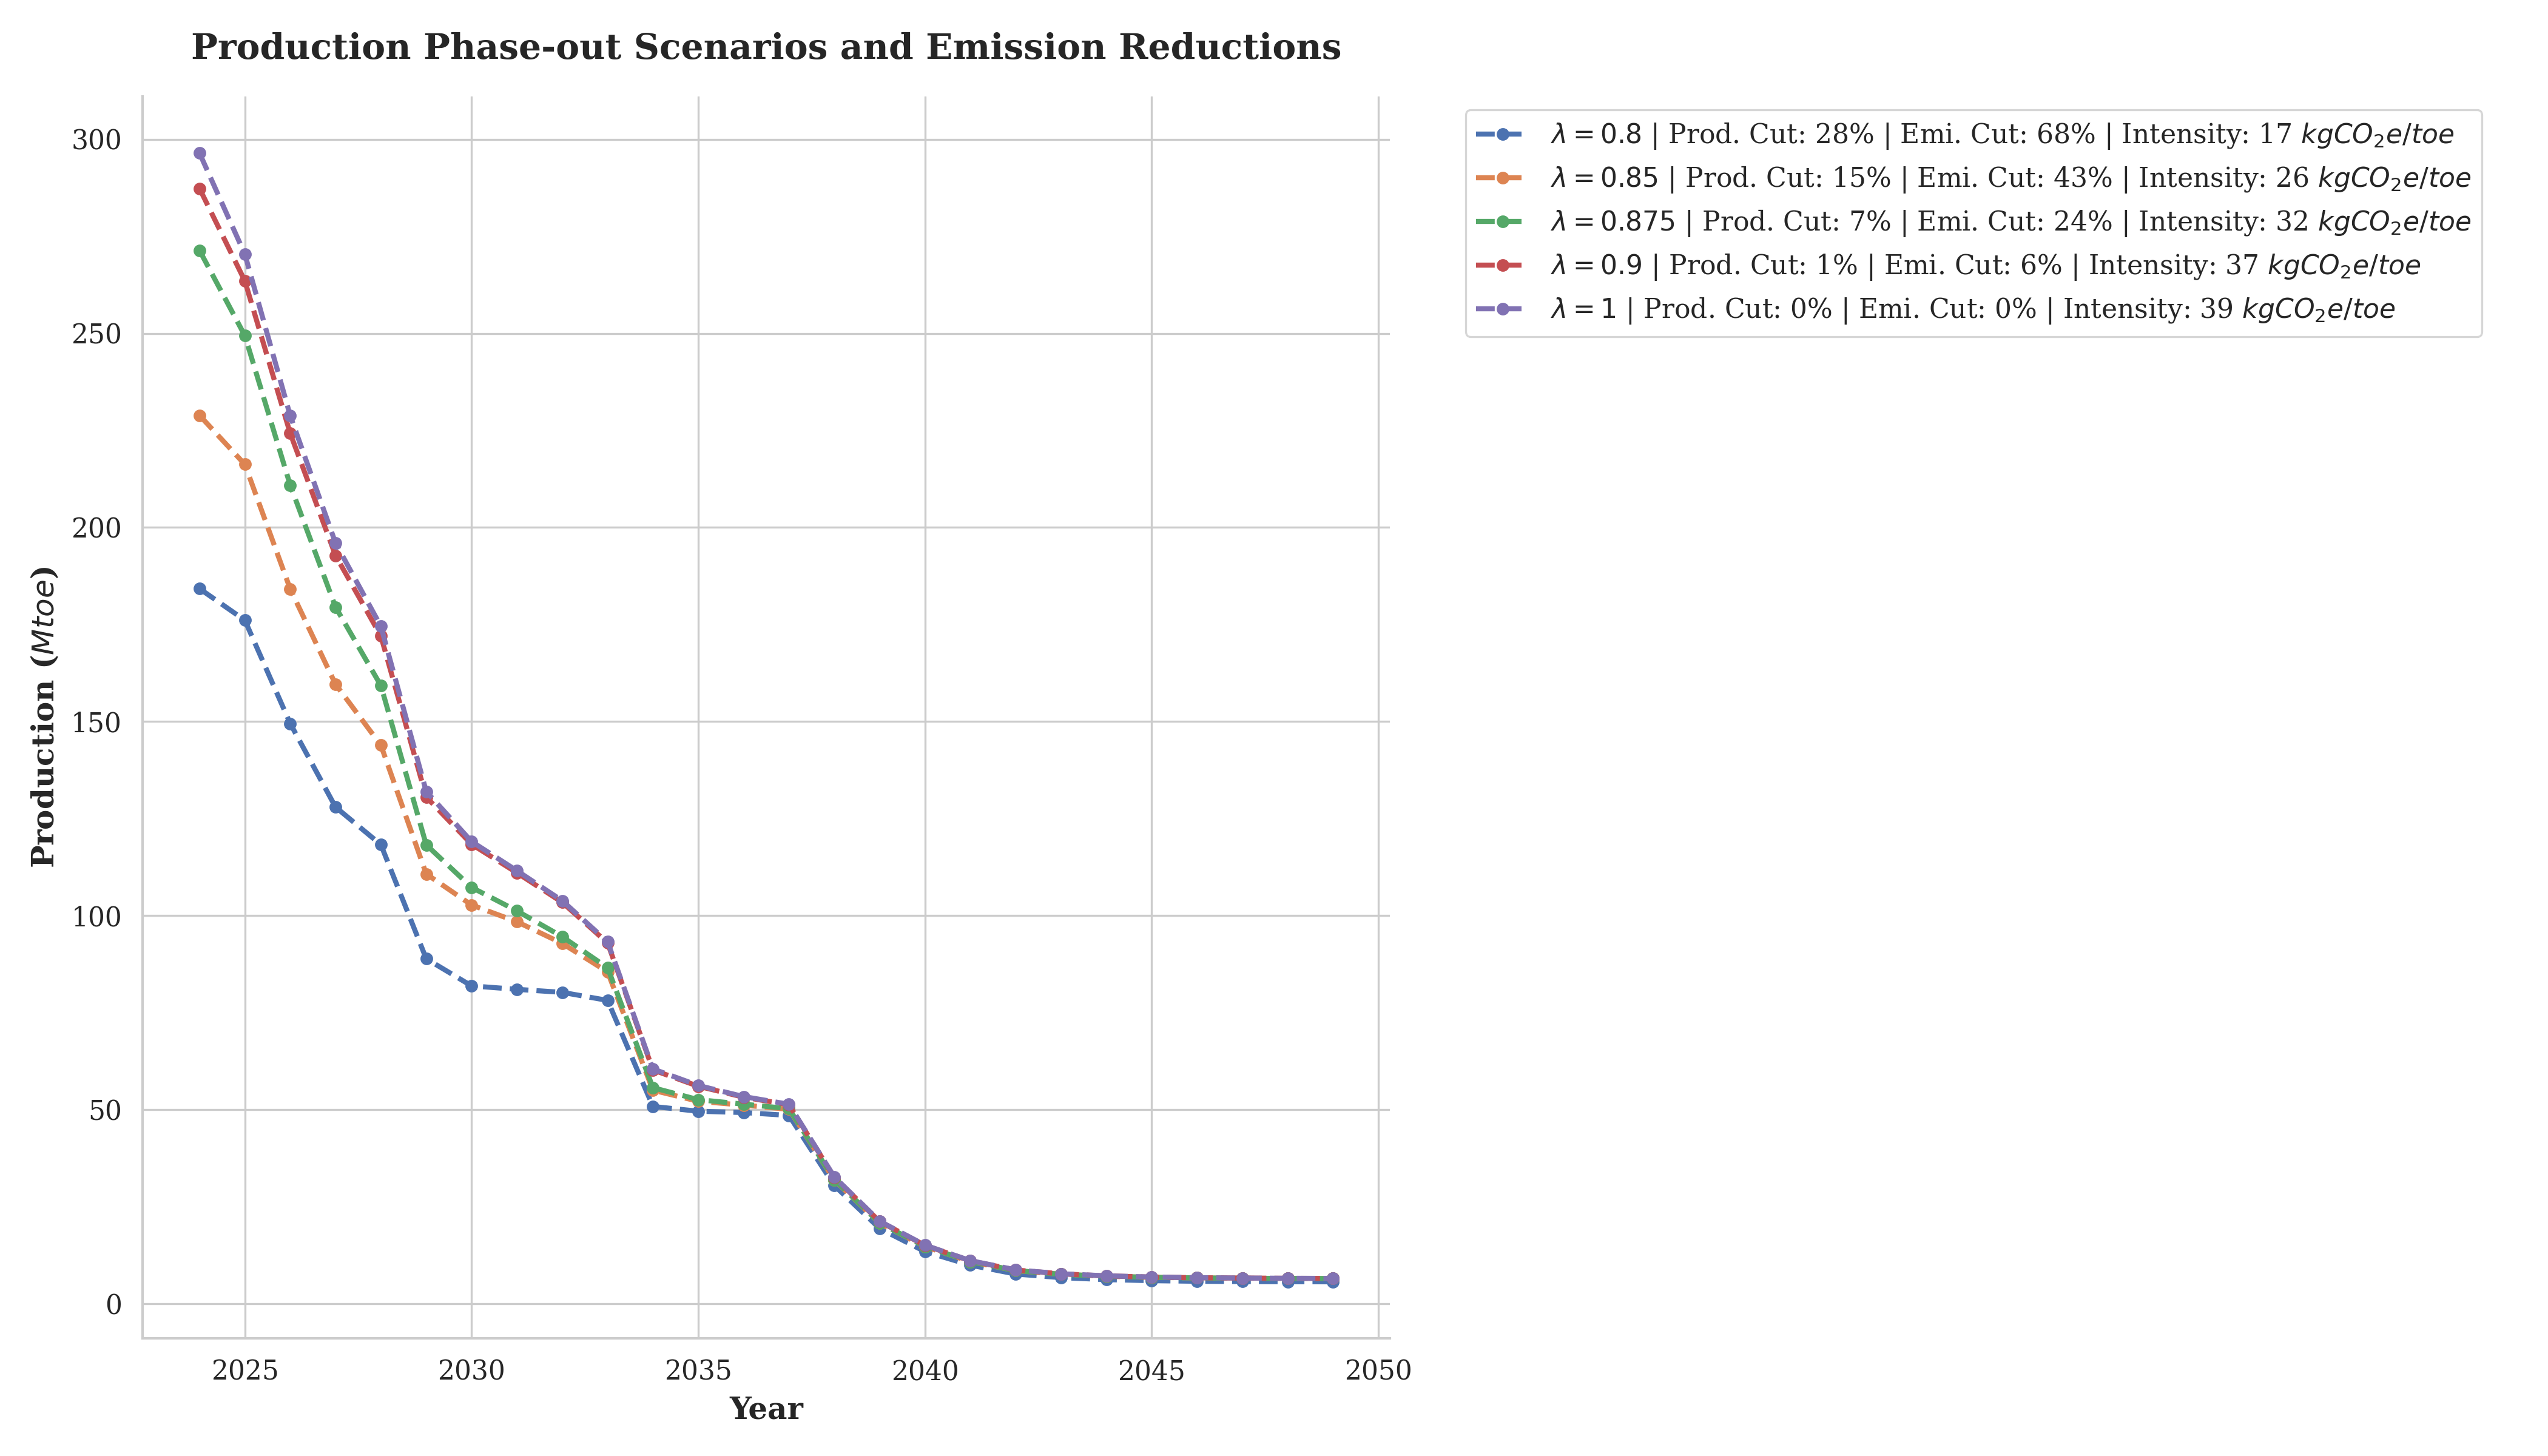
\includegraphics[keepaspectratio,alt={Production Phase-out Scenarios}]{../production_scenarios.png}}
\caption{Production Phase-out Scenarios}
\end{figure}

\subsubsection{Case Studies in Phase-Out
Dynamics}\label{case-studies-in-phase-out-dynamics}

By restricting the stringency parameter \(\lambda\), the algorithm
sequentially shuts down the most inefficient fields: - \textbf{Immediate
Closure (Statfjord \& Brage):} At a modest \(\lambda = 0.9\) (a 10\%
emission cut), the model immediately sacrifices late-life fields like
Statfjord and Brage. These fields have immense legacy infrastructure but
highly depleted reservoirs, making their marginal carbon intensity
unacceptably high. - \textbf{Resilient Core (Edvard Grieg \& Johan
Sverdrup):} Conversely, newer fields equipped with modern extraction
technology and high initial reservoir pressures are protected by the
algorithm even under extreme \(\lambda = 0.5\) constraints, as they
provide massive economic yield for minimal carbon overhead.

\begin{figure}
\centering
\pandocbounded{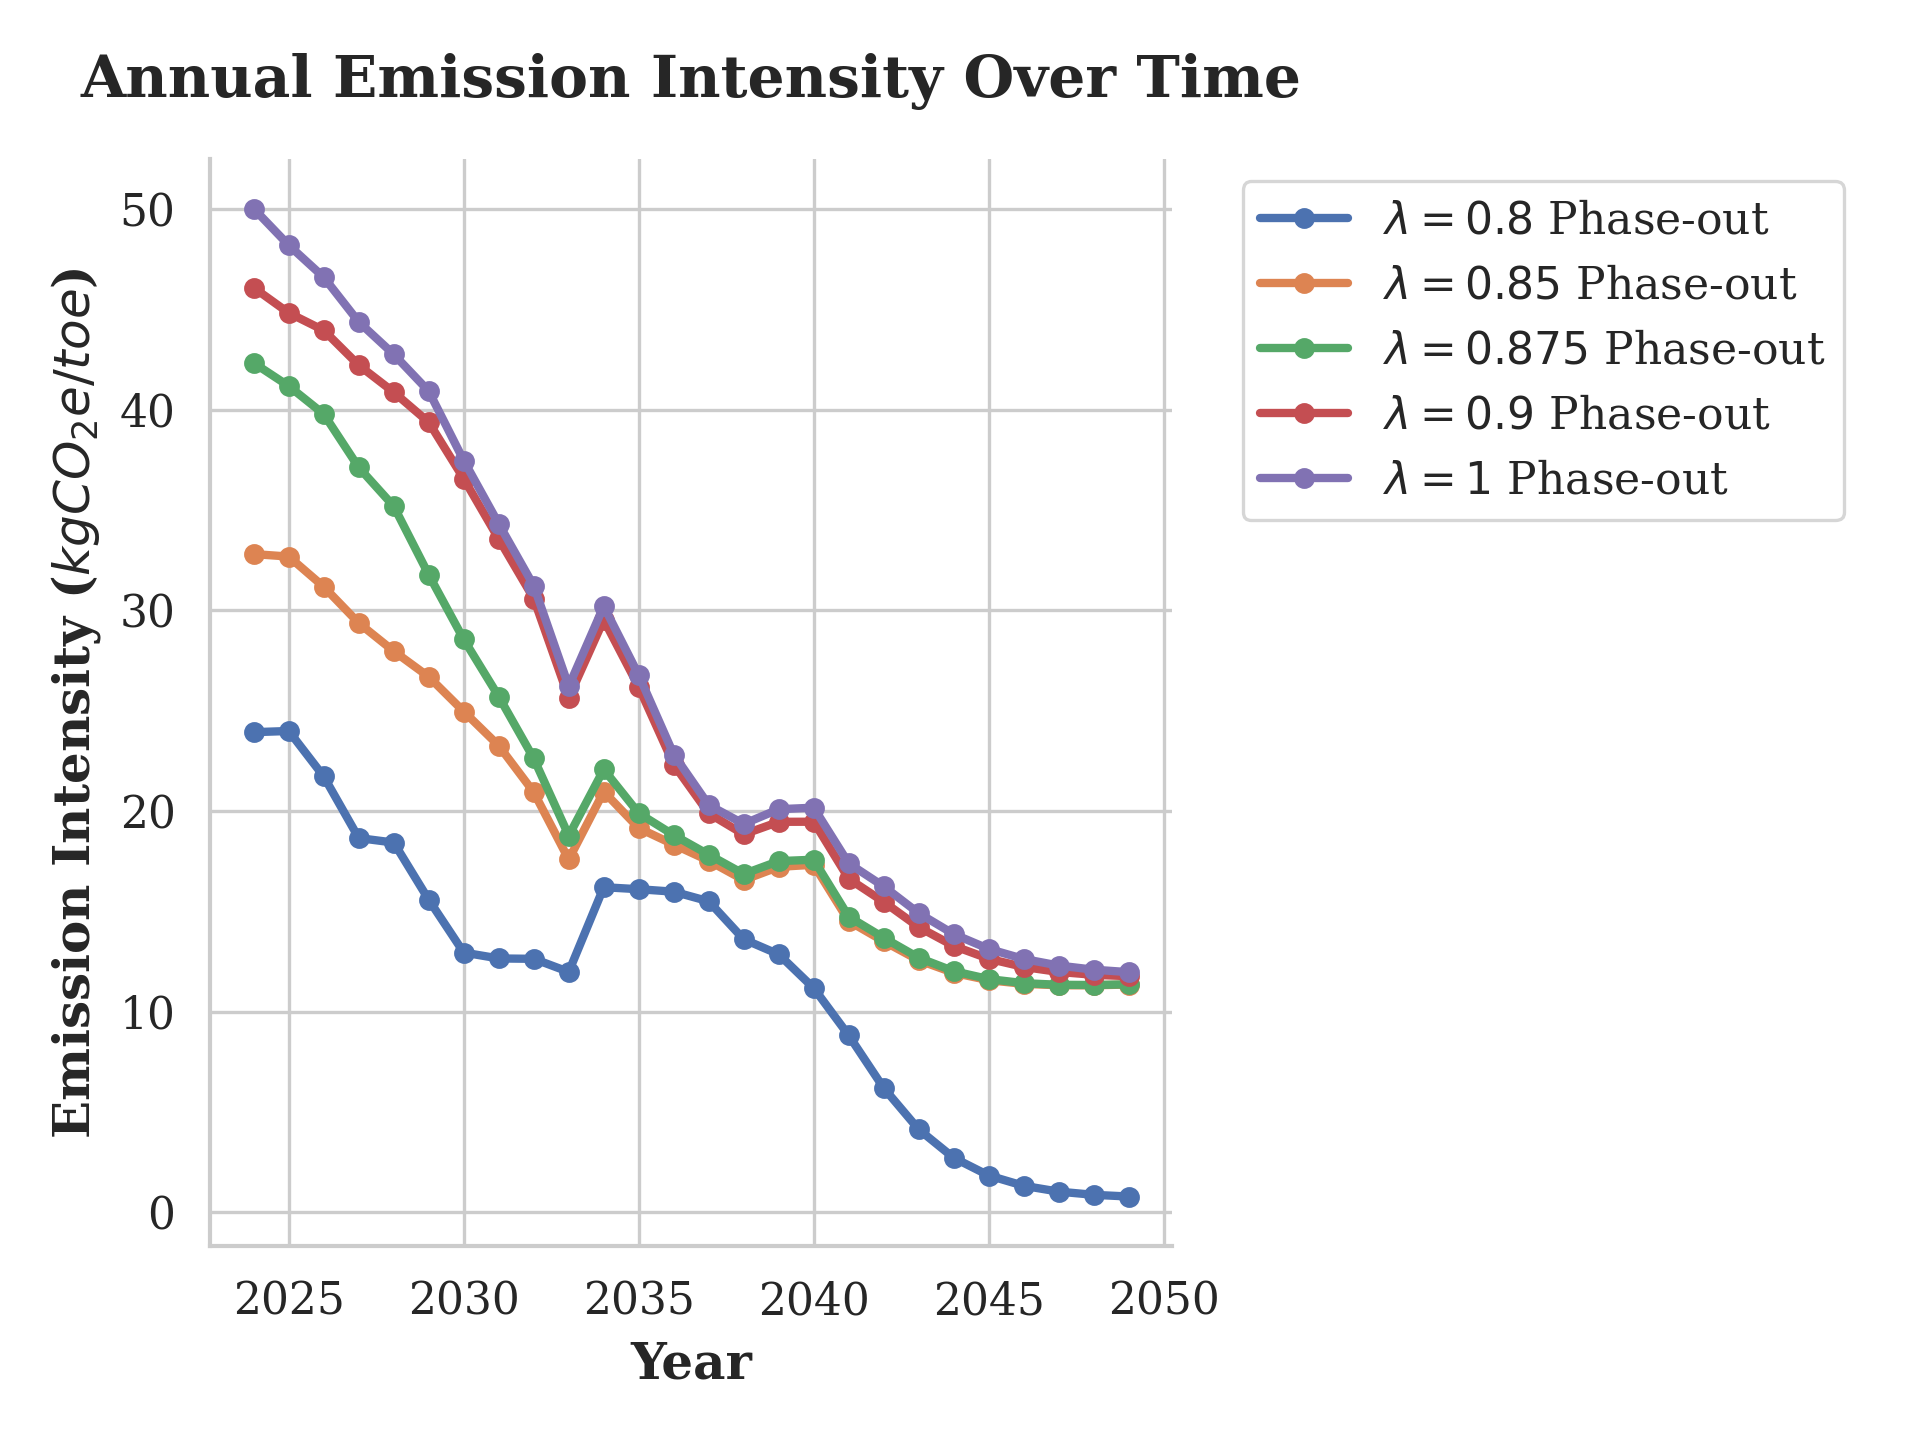
\includegraphics[keepaspectratio,alt={Annual Emission Intensity}]{../annual_intensity.png}}
\caption{Annual Emission Intensity}
\end{figure}

\subsection{4.4. Marginal Abatement Cost
(MAC)}\label{marginal-abatement-cost-mac}

The MAC curve derived from our optimization clearly illustrates the
economic efficiency of the targeted phase-out. Initial emission
reductions (the first 20\%) can be achieved at near-zero marginal cost
by closing highly inefficient tail-end producers.

However, the curve steepens dramatically. To meet deeper decarbonization
targets beyond 30\%, the algorithm is forced to shut down younger,
highly profitable fields. At this critical inflection point, the lost
revenue per ton of CO2 abated skyrockets, severely testing the political
viability of pure phase-out strategies in the current energy-secure
macroeconomic climate.

\begin{figure}
\centering
\pandocbounded{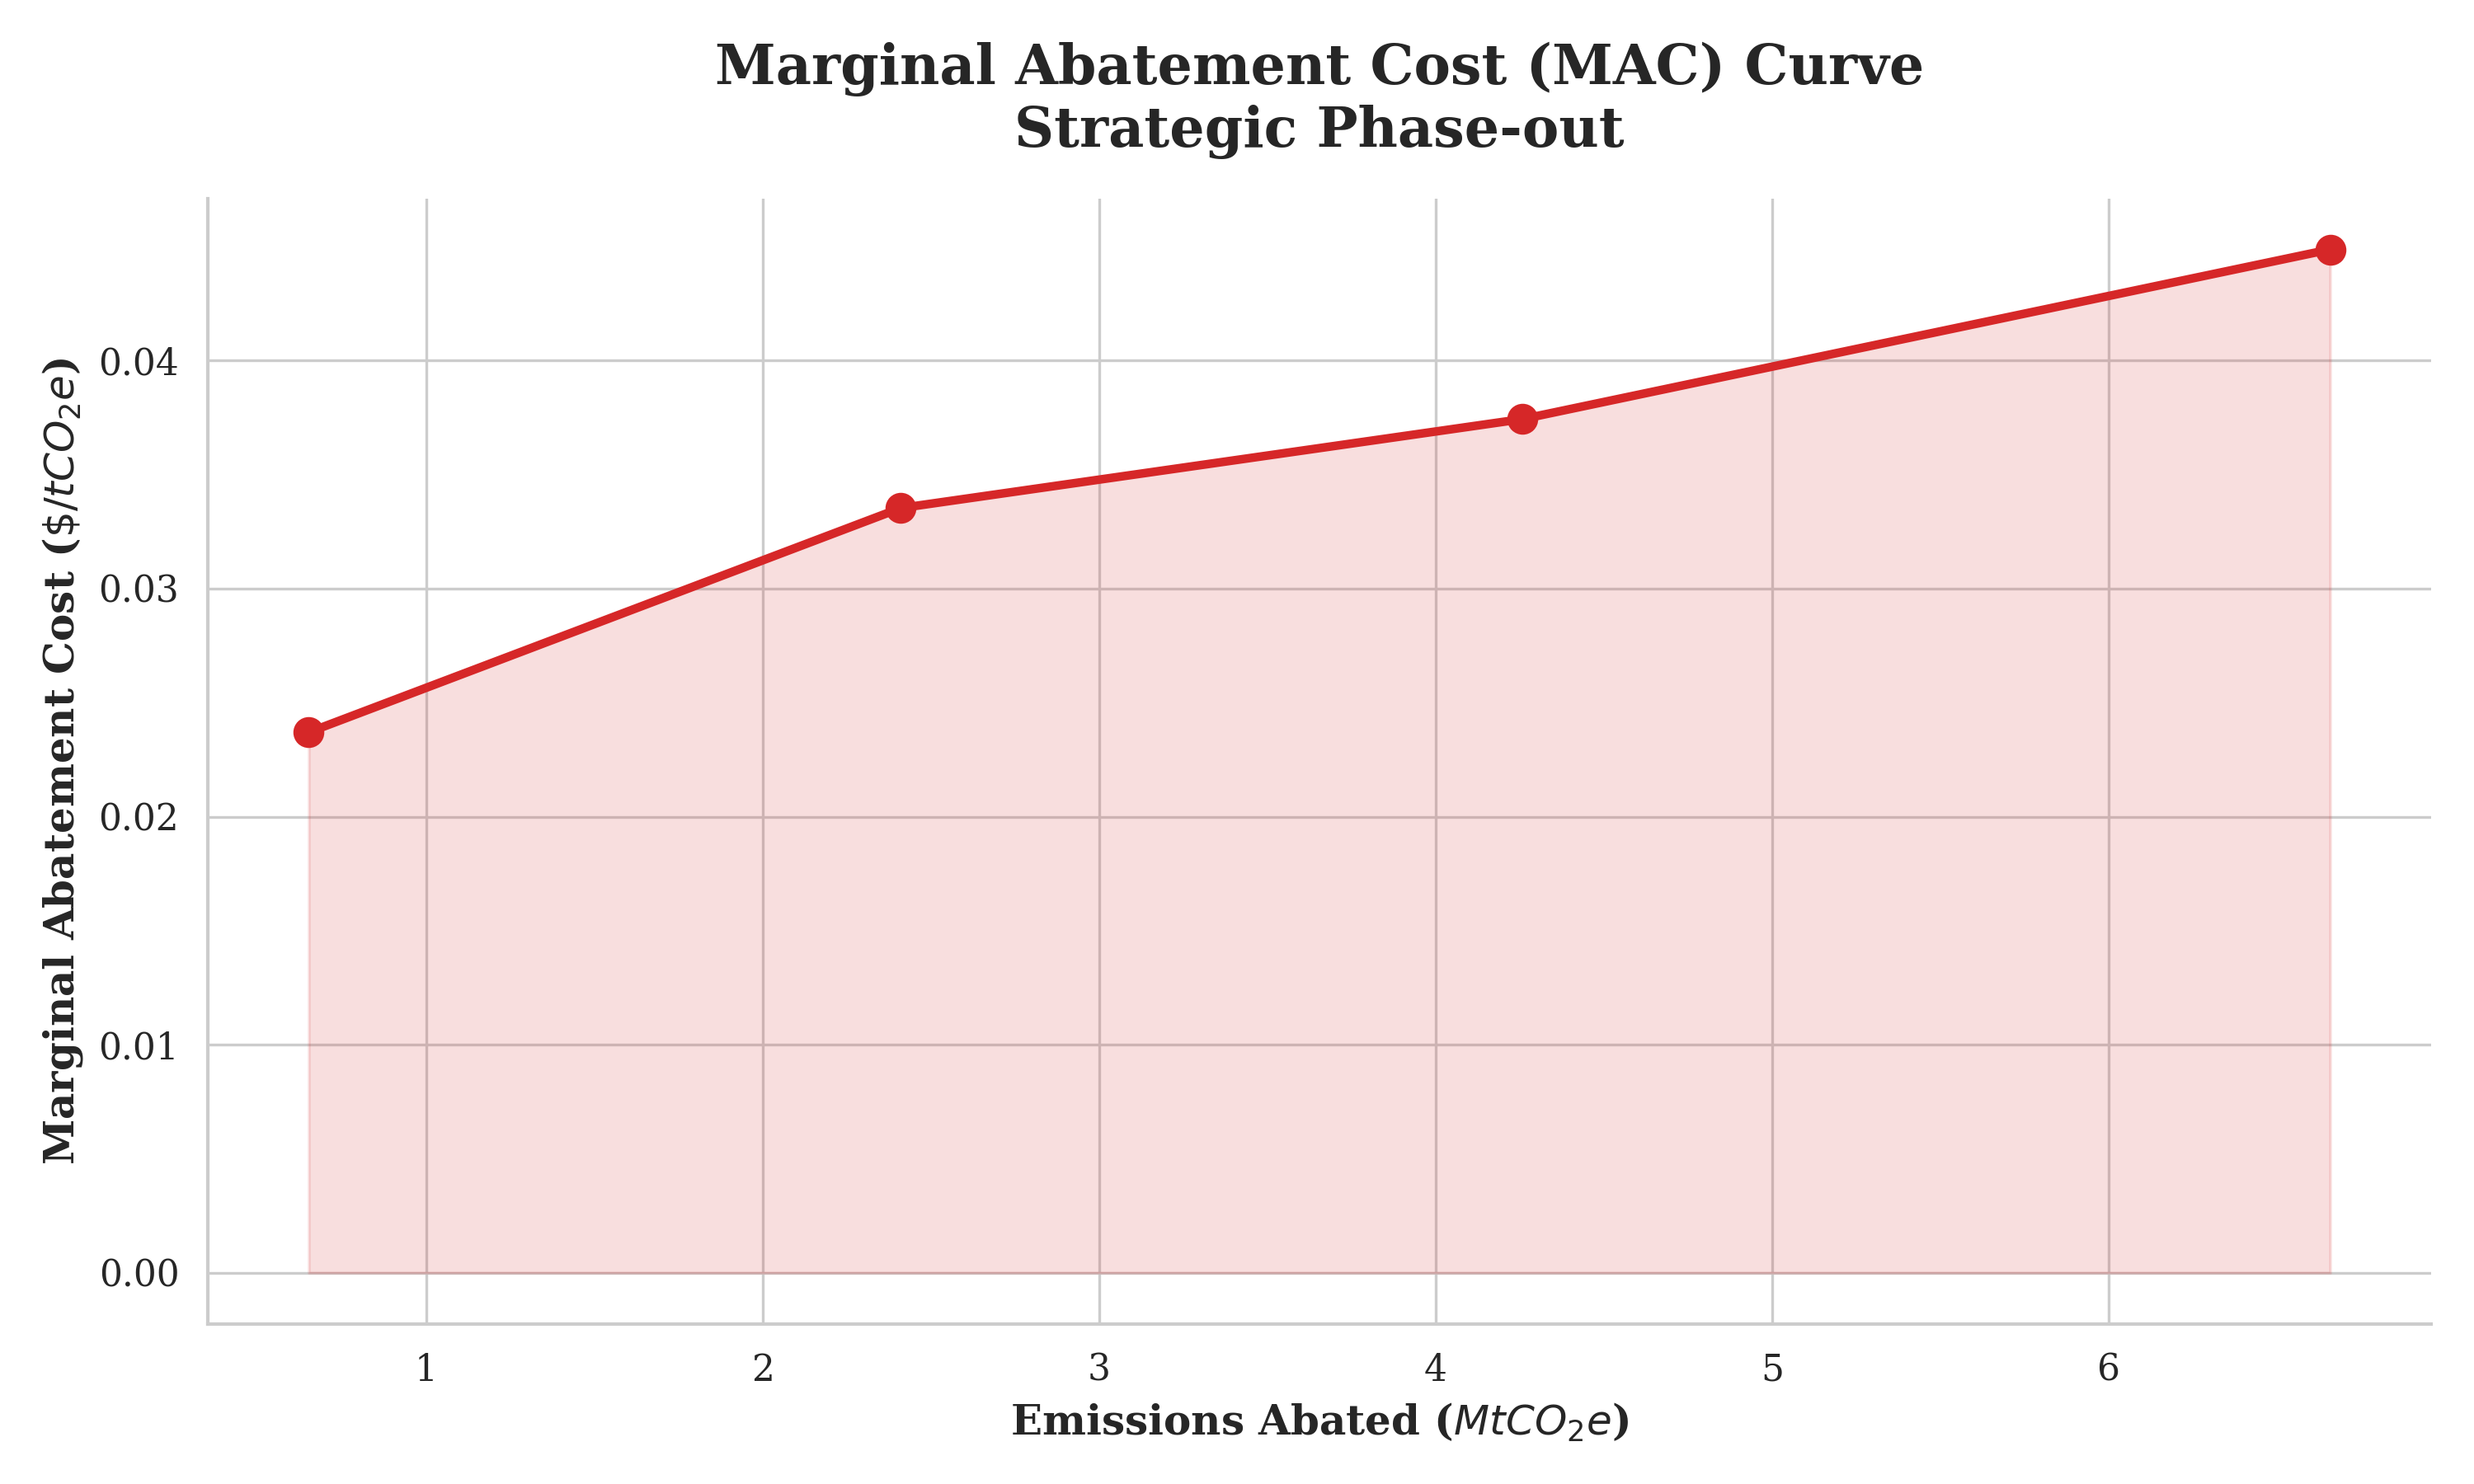
\includegraphics[keepaspectratio,alt={Marginal Abatement Cost Curve}]{../mac_curve.png}}
\caption{Marginal Abatement Cost Curve}
\end{figure}

\begin{center}\rule{0.5\linewidth}{0.5pt}\end{center}

\section{5. Discussion}\label{discussion}

As the 2030 ``Fit For 55'' deadline rapidly approaches, the Norwegian
Continental Shelf operates at the epicenter of a profound macroeconomic
conflict. On one side, severe geopolitical instability following the
events of the mid-2020s has positioned Norwegian gas as the
indispensable backbone of European energy security. On the other side,
domestic climate mandates demand an immediate and brutal reduction in
offshore carbon intensity.

Our data-driven algorithmic optimization proves that broad-stroke,
top-down policies---such as uniform carbon taxation---are mathematically
suboptimal in this environment. The extreme heterogeneity of offshore
assets means that flat carbon prices fail to effectively phase out the
highest polluters, instead merely eroding the margins of highly
efficient, modern fields like Johan Sverdrup.

By utilizing Double Machine Learning to identify the true causal drivers
of carbon intensity, we empower a surgical policy approach. Our linear
programming models demonstrate that electrifying just 13 specific hubs
or selectively shutting down a small cohort of highly depleted tail-end
fields (sacrificing 28\% of future production) can successfully meet the
55\% reduction mandate.

However, the Marginal Abatement Cost (MAC) curve reveals a sharp
inflection point. While the initial 20\% of emissions can be abated
cheaply by retiring inefficient legacy infrastructure, pushing beyond a
30\% reduction via phase-outs incurs astronomical economic losses,
jeopardizing European energy supply. In the volatile political climate
of May 2026, policymakers must therefore carefully weigh the
mathematical efficiency of targeted electrification against the
political resistance to onshore grid expansion.

Ultimately, this paper provides a robust, replicable, and dynamic
framework for algorithmic climate policy, ensuring that the necessary
decarbonization of the offshore energy sector is achieved with
mathematical precision and maximal economic resilience.

\subsubsection{Limitations}\label{limitations}

While our DML framework controls for observed confounders, proprietary
data regarding field-specific operating costs (OPEX) and exact
electrification capital expenditures (CAPEX) remains limited. Future
research should integrate high-resolution financial data to refine the
MAC curve from a proxy-based estimate to an exact economic forecast.

\subsubsection{Conclusion}\label{conclusion}

By integrating granular geospatial data with Double Machine Learning and
constrained optimization, we provide a replicable blueprint for
decarbonizing mature oil and gas basins. Our models suggest that the
``Fit For 55'' targets are achievable on the NCS, provided that policy
mechanisms correctly target the extreme variance in field-level carbon
intensity.

\begin{center}\rule{0.5\linewidth}{0.5pt}\end{center}

\section{References}\label{references}

\begin{enumerate}
\def\labelenumi{\arabic{enumi}.}
\tightlist
\item
  \textbf{Chernozhukov, V., Chetverikov, D., Demirer, M., Duflo, E.,
  Hansen, C., Newey, W., \& Robins, J.} (2018). \emph{Double/debiased
  machine learning for treatment and structural parameters}. The
  Econometrics Journal, 21(1), C1-C68.
\item
  \textbf{European Commission.} (2021). \emph{`Fit for 55': delivering
  the EU's 2030 Climate Target on the way to climate neutrality}.
  COM/2021/550 final.
\item
  \textbf{Norwegian Petroleum Directorate.} (2025). \emph{Resource
  Report 2024: Energy transition on the Norwegian Continental Shelf}.
\item
  \textbf{Nordhaus, W. D.} (2017). \emph{Revisiting the social cost of
  carbon}. Proceedings of the National Academy of Sciences, 114(7),
  1518-1523.
\item
  \textbf{Gillingham, K., \& Stock, J. H.} (2018). \emph{The cost of
  reducing greenhouse gas emissions}. Journal of Economic Perspectives,
  32(4), 53-72.
\item
  \textbf{IEA.} (2024). \emph{The Role of Critical Minerals in Clean
  Energy Transitions}. World Energy Outlook Special Report.
\item
  \textbf{Knittel, C. K., \& Metaxoglou, K.} (2014). \emph{Estimation of
  structural industrial organization models: A guide for practitioners}.
  Journal of Applied Econometrics, 29(2), 301-317.
\item
  \textbf{Pearl, J.} (2009). \emph{Causality: Models, Reasoning, and
  Inference}. Cambridge University Press.
\item
  \textbf{Sokkeldirektoratet.} (2026). \emph{Annual Emissions and
  Production Inventory for the NCS}.
\end{enumerate}

\begin{center}\rule{0.5\linewidth}{0.5pt}\end{center}

\end{document}
